\label{sec:Squeezers}

\subsection{Squeezed light sources}

\bluecomment{SS: should this section move to after the next one, i.e. after the discussion of quantum-noise reduction techniques?}

Squeezed states of light \cite{Yuen76,Walls1983,Breitenbach97} provide a way of increasing the sensitivity of a gravitational wave detector in the quantum noise limited region, independently of the circulating light power. Generally, a light field is described by two non-commuting physical quantities, the amplitude and phase quadratures. The minimum product of their uncertainties is limited by Heisenbergs uncertainty relation, which is also valid in the complete absence of photons, that is for a vacuum state. Vacuum states as well as coherent states have noise equally distributed in the field quadratures. Squeezed states show a noise below the vacuum noise level, however, owing to the Heisenberg uncertainty principle, this is not possible for all quadratures of the state simultaneously.  

For a Michelson interferometer operated close to a dark output port, squeezed states can be used by injecting them into the signal port and spatially overlapping them with the high power laser field at the beam splitter \cite{1981_PRD.23.1693_Caves}. The squeezed quadrature has to be controlled such that, after being reflected off the interferometer, it is in phase with the readout (amplitude) quadrature of the observatory output light. For reviews on the application of squeezed states of light in the framework of gravitational wave detectors we refer to Refs. \cite{Schnabel2010,Schnabel2017,Barsotti2018}.

Squeezing has a significant impact if large squeezing factors can be produced and detected. For example, an effective squeezing level of 3\,dB improves the signal-to-noise ratio by a factor of $\sqrt{2}$ at shot-noise limited frequencies, which is equivalent to doubling the interferometer's input laser power. An effective squeezing level of 10\,dB would correspond to a ten-fold power increase. Here, effective squeezing does not refer to the injected squeezing initially available, but rather describes the quantum noise reduction measurable with the photo detector(s) at the observatory's output.  
%
Any optical loss between squeezing generation and detection reduces the level of measurable squeezing. Therefore, a prerequisite for the 10\,dB of effective squeezing envisaged for ET, is a squeezed light source design that can provide sufficiently strong squeezed vacuum states of light at the expected gravitational wave signal frequencies ranging from 10 Hz to 10 kHz. 

Significant progress has been made over the last 10 years in the generation of squeezed vacuum states of light and squeeze factors beyond 10\,dB are routinely produced at the two required wavelengths, 1064 nm and 1550 nm, respectively.
%
In the same manner as today's most efficient squeezed light sources, the ET-squeezers will employ cavity-enhanced parametric down-conversion, also called optical parametric amplification, where the interaction between the fundamental and second harmonic fields via a $\chi^{(2)}$-process inside a non-linear crystal produces non-classical photon-pair correlations that yield a reduced noise variance in a certain field quadrature.  
%
%Cavity enhanced squeezed light generation can be realized with different optical topologies.  
%
%
\begin{figure} %[htbp]
\centering
{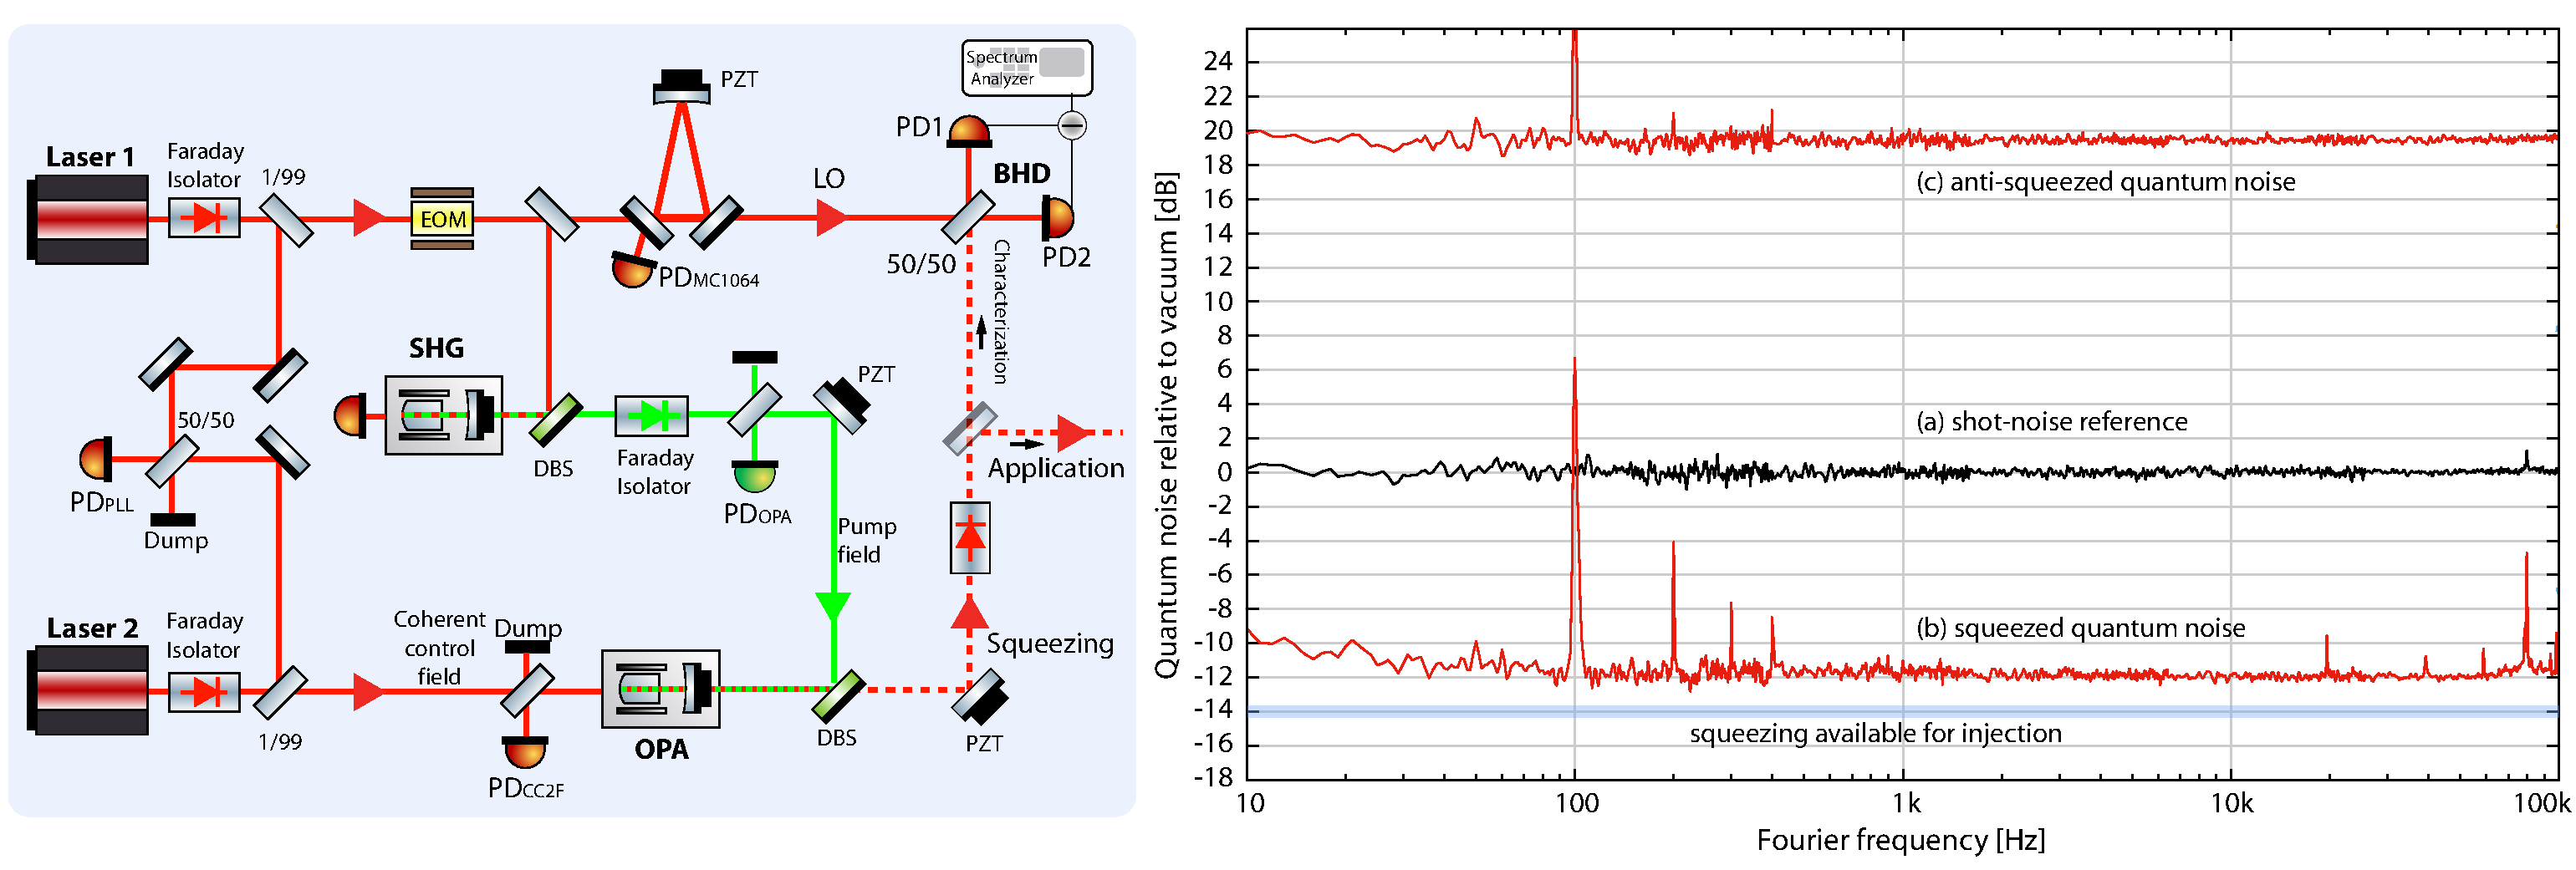
\includegraphics[width=\linewidth]{Detector/DetFigures/SqueezerFig1b.pdf}}
\caption{{\bf{Left:}} Schematic for the generation and coherent control of squeezed vacuum states of light. Laser 1 provides the light field for homodyne detection and for frequency doubling in a second harmonic generator (SHG). The SHG provides the pump field required for the generation of squeezed vacuum states in an optical parametric amplifier (OPA) operated below threshold. The squeezed vacuum states are extracted via a dichroic beam splitter (DBS) and send towards the interferometer. Alternatively, the squeezing level can be characterized by means of a balanced homodyne detector (BHD).  A Faraday isolator is implemented in the squeezing path to protect the OPA from light scattered back from the interferometer.\\
{\bf{Right}}: Quantum noise squeezing as reported in \cite{Mehmet2018}. Trace (a) represents the shot noise reference (normalized to 0\,dB) measured with a homodyne detector. In reference to this trace the measured quantum noise powers for squeezing (b) and the corresponding anti-squeezing (c) are shown.
Up to 12\,dB squeezing and 19.6\,dB anti-squeezing was observed, which is consistent with a theoretical model assuming a residual phase noise of 3.5\,mrad rms and an overall optical loss of 5.3\,\% for the squeezed field. This includes 2.5\,\%  optical loss due to the homodyne detection which needs to be subtracted to deduce the squeezing level available for the injection into a gravitational wave detector. This level is indicated by the blue area and corresponds to a squeezing factor of 14\,dB.}
\label{SqueezerFig1}
\end{figure}
%
The strongest squeezing level demonstrated to date is a squeeze factor of 15\,dB below the classical shot-noise limit at the wavelength of 1064\,nm, but only measured at MHz frequencies~\cite{Vahlbruch2016}. The topology of the optical parametric amplifier (OPA) used therein was a linear, standing-wave, doubly-resonant cavity with a non-linear crystal made from periodically poled potassium titanyl phosphate (PPKTP).  
%
Up to 13\,dB of non-classical noise suppression was measured at a wavelength of 1550\,nm~\cite{Schonbeck18} in a similar cavity design, but again only at MHz frequencies. 
%
By the implementation of a coherent control scheme \cite{Vahlbruch2006} and the mitigation of parasitic interferences the frequency band of detectable squeezing can be extended from MHz down to the required GW-frequencies \cite{Vahlbruch2007}. 
This has been demonstrated in tabletop experiments with various squeezed light source setups operated in-air or in-vacuum and with OPAs constructed as bow-tie or linear resonators \cite{Vahlbruch2006,Stefszky2012, Wade2016}.
%
Following these developments, similar schemes were used to realize squeezing enhancement in large scale gravitational wave detectors. 
The first successful implementation was achieved at the GEO600 detector in 2010 and since then squeezing has been routinely applied \cite{2011_Nat.Phys.7.962_LSC, Grote2013}. 
The Advanced Virgo and the two Advanced Ligo detectors have been also upgraded to include the squeezing technique since the O3 science run in early 2019.  
%

The most efficient \bluecomment{SS: what's efficient in this context, and/or is it relevant?} squeezed light source at GW-frequencies so far was reported in 2018 \cite{Mehmet2018} at AEI Hannover. Figure \ref{SqueezerFig1} summarizes the main result of this work, where squeezed light was generated in a linear, doubly-resonant OPA at a wavelength of 1064\,nm. A quantum noise reduction of up to 12\,dB at Fourier frequencies between 10\,Hz and 100\,kHz was directly measured with a diagnostic homodyne detector. The analysis revealed that the measured squeezing level corresponds to an equivalent squeezing factor of up to 14\,dB available for the injection into a gravitational wave detector with only 3.5\,mrad rms of phase noise attributed to the squeezed light source operated in air \bluecomment{SS: how does this compare to the assumed effective squeezing level of 10dB of Table3.1? Maybe link to Fig 3.7 to show that phase noise at that level should give sufficient margin.}. The recent progress in the development of low-loss Faraday isolators suggests that this squeezing factor can be even further improved in the near future \bluecomment{SS: reference? Is this also valid for 1550nm?}. 
At the wavelength of 1550\,nm there are also so far no indications why a comparably high squeezing level should not be observable \bluecomment{SS: double-negative makes this a bit hard to read} at GW-detection-frequencies once a coherent control scheme is implemented \cite{Mehmet2011} \bluecomment{SS: I'm not aware of any (citeable) progress in that direction, but it feels like there should be.}. 

\bluecomment{SS: with the 532nm pump light, degradation of optics/crystals over time seems to be an issue. Has there been progress on this or are concepts foreseen that might reduce downtime? Do we expect better long-term performance at 775nm?}
Based on the demonstrated technical readiness, a total of six independent squeezed light sources will be engineered for ET: Three systems will generate squeezing at 1550\,nm for the ET-LF detector and three systems operating at 1064\,nm will be used for the ET-HF detectors. 
